\Def Хроматическое число пространства - min количество цветов, в которое можно так покрасить все точки этого пространства, чтобы между точками одного цвета не было расстояния 1:

$\chi(\R^n) = min \{\chi: \R^n = V_1 \sqcup V_2 \sqcup \dots \sqcup V_{\chi} : \forall i, \forall \overline{x}, \overline{y} \in V_i |\overline{x} - \overline{y}| \neq 1 \}$

\Example $\chi(\R) = 2$, просто красим полуинтервалы длины 1 в разные цвета.

\Th $\chi(\R^n) \geqslant (c + o(1))^{dim}$

\Proof
$G(n, 3, 1)$ - граф из 9 билета. Очевидно, что $\chi(\R^n) \geqslant \chi(G(n, 3, 1)) \geqslant \frac{|V|}{\alpha(G(n, 3, 1))} = \frac{C_n^3}{m(n, 3, 1)} \geqslant \frac{C_n^3}{n} \sim \frac{n^2}{6} $. 

Теперь перейдём к более общему случаю $G(n, r, s)$:

$\chi(\R^n) \geqslant \chi(G(n, r, s)) \geqslant \frac{C_n^r}{m(n, r, s)}$

Заметим, что расстояние между двумя рёбрами $G(n, r, s)$ равно $\sqrt{2(r-s)}$ (просто расписать расстояние между векторами).

Теперь максимизируем правую дробь. Возьмём $r = r(n) \sim \frac{2 - \sqrt{2}}{2} \cdot n$ (можно сделать r целой частью от этой же штуки), $s\sim \frac{r}{2}$
Это расстояние должно быть простым числом $p$. Из курса ОКТЧ мы всегда можем выбрать простое число в отрезке $[x, x+O(x^{0.525})]$ при достаточно больших значениях, т.е. мы найдём подходящее нам простое число.

$\frac{C_n^{[\frac{2 - \sqrt{2}}{2}]}}{\sum_{k=0}^{p-1} C_n^k}$

$a = \frac{2 - \sqrt{2}}{2}$, тогда 

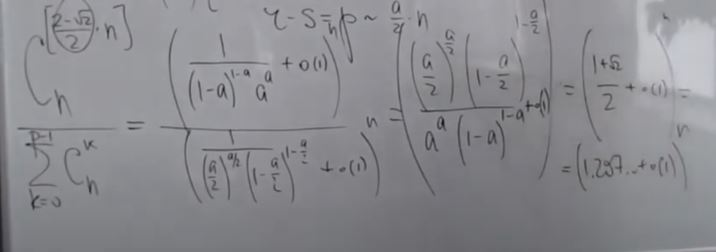
\includegraphics[]{images/71_2.JPG}
\EndProof